

\tikzset{every picture/.style={line width=0.75pt}} %set default line width to 0.75pt        

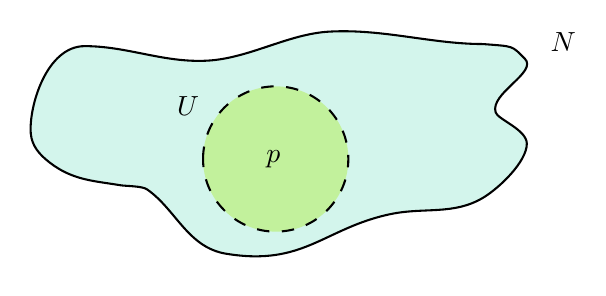
\begin{tikzpicture}[x=0.75pt,y=0.75pt,yscale=-1,xscale=1]
%uncomment if require: \path (0,203); %set diagram left start at 0, and has height of 203

%Curve Lines [id:da28281619681811754] 
\draw [fill={rgb, 255:red, 211; green, 245; blue, 236 }  ,fill opacity=1 ][line width=0.75] [line join = round][line cap = round]   (264,41.63) .. controls (239.07,41.63) and (216.02,34.24) .. (190,35.63) .. controls (169.94,36.71) and (151.25,48.57) .. (131,49.63) .. controls (109.98,50.74) and (92.57,42.63) .. (72,42.63) .. controls (53.59,42.63) and (45.01,71.73) .. (46,84.63) .. controls (46.47,90.7) and (50.18,94.88) .. (55,98.63) .. controls (66.08,107.25) and (76.24,107.51) .. (89,109.63) .. controls (91.95,110.13) and (99.58,109.96) .. (102,111.63) .. controls (115.88,121.24) and (121.56,139.56) .. (140,142.63) .. controls (177.55,148.89) and (187.14,130.46) .. (219,123.63) .. controls (235.52,120.09) and (249.69,124.22) .. (264,115.63) .. controls (271.71,111.01) and (285,98.32) .. (285,89.63) .. controls (285,82.9) and (271.1,77.94) .. (270,74.63) .. controls (266.91,65.36) and (290.59,55.22) .. (284,48.63) .. controls (277.54,42.17) and (279,42.85) .. (264,41.63) -- cycle ;
%Shape: Circle [id:dp001327175657310109] 
\draw  [fill={rgb, 255:red, 194; green, 241; blue, 156 }  ,fill opacity=1 ][dash pattern={on 4.5pt off 4.5pt}] (129,97) .. controls (129,77.67) and (144.67,62) .. (164,62) .. controls (183.33,62) and (199,77.67) .. (199,97) .. controls (199,116.33) and (183.33,132) .. (164,132) .. controls (144.67,132) and (129,116.33) .. (129,97) -- cycle ;

% Text Node
\draw (158,91.4) node [anchor=north west][inner sep=0.75pt]    {$p$};
% Text Node
\draw (115,65.4) node [anchor=north west][inner sep=0.75pt]    {$U$};
% Text Node
\draw (295,34.4) node [anchor=north west][inner sep=0.75pt]    {$N$};


\end{tikzpicture}
